\paragraph{Gestione profilo utente}

\label{Gestione profilo utente}

\begin{figure}[ht]
	\centering
	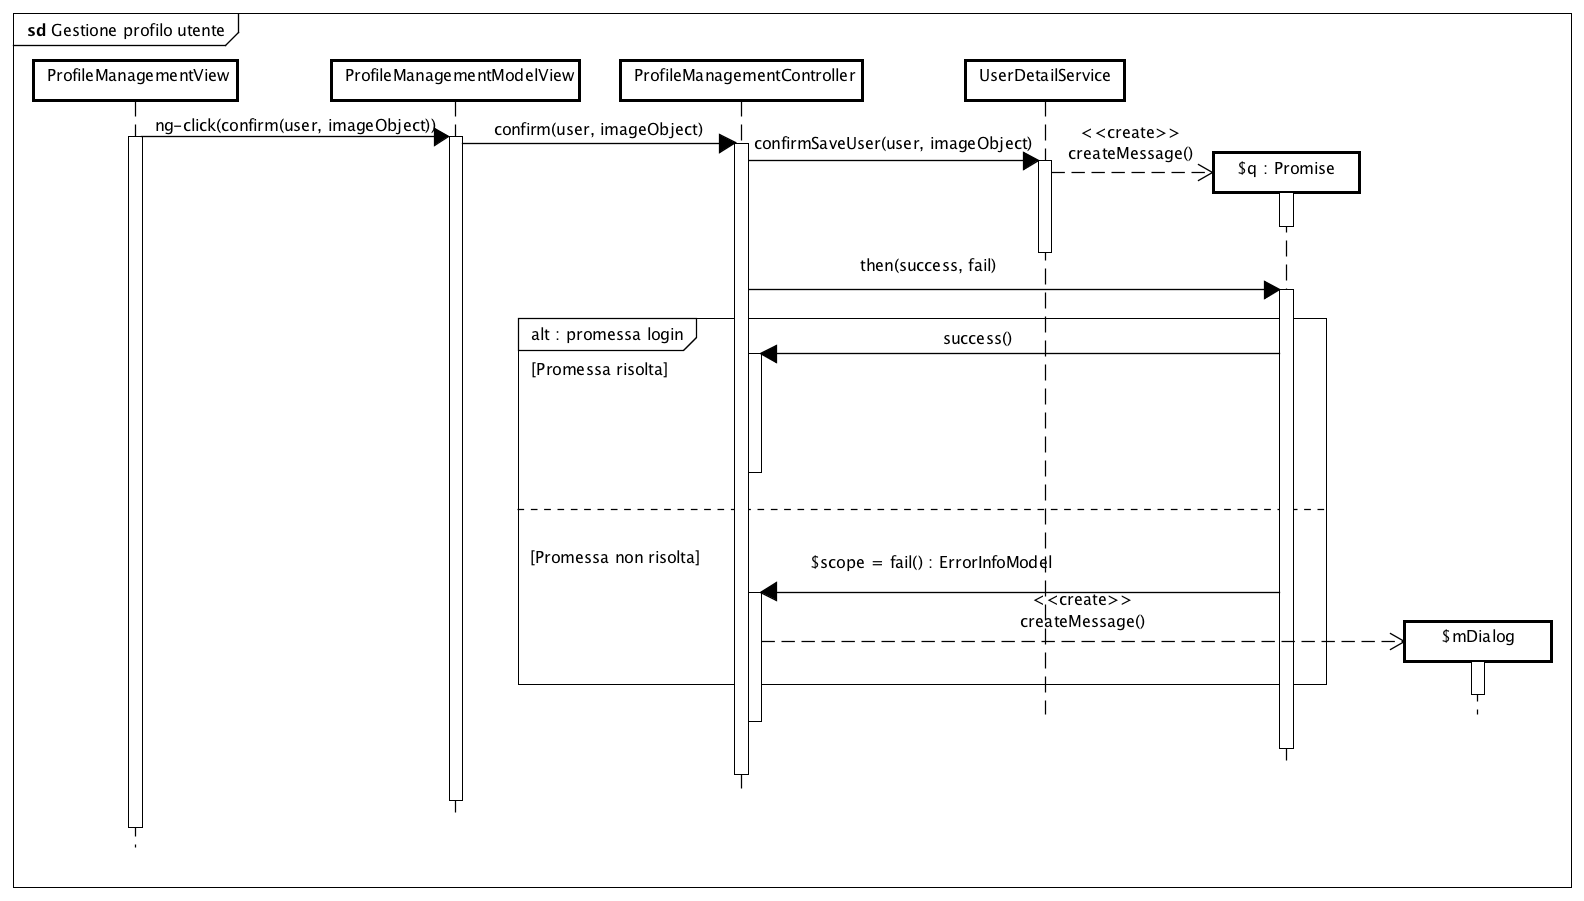
\includegraphics[scale=0.375,keepaspectratio]{UML/DiagrammiDiSequenza/Front-end/ProfileManagement.png}
	\caption{Gestione profilo utente}
\end{figure} \FloatBarrier

L'utente può modificare i suoi dati personali cambiando le informazioni dai campi dati presenti in \texttt{ProfileManagementView} e rendere persistenti tali modifiche avviando l'evento associato al bottone presente in tale \textit{view\ped{G}}. Il \texttt{ProfileManagementController} gestisce l'evento chiamando il metodo \texttt{confirm} dell'\texttt{AuthService}, il quale restituirà una conferma. Se la promessa viene soddisfatta vengono rese persistenti le modifiche dei dati, altrimenti  verrà restituito un oggetto di tipo \texttt{ErrorInfoModel} e mostrato a video mediante \texttt{\$mdDialog}. 